\chapter{Project Analysis}
\label{chap:prjan}

\section{Project Scheduling}
\label{chap:prjan:sec:prjsche}

Before starting this project a time requirements has been carried out, to see
its feasibility. We calculated at least six month necessary to be able to create
a working proof of concept (PoC) that allowed us to perform tests and, in
general, to have a feedback about the solution.

\subsection{Scheduled timeline}
Since our knowledge about the technologies was very poor at the beginning, we
preferred to invest a good chunk of time on studying them, to understand the already
present products available in the market and to choose what we really needed.
Additionally, at the end of this phase we though it was necessary to try these
products to see if they really fitted our necessities. After this phase, we
planned to actually starting implementing the missing components to create and
to fulfill the requirements defined in Section~\ref{chap:prjan:sec:req}. Since
the required technologies, Java and C/C++ are known to the authors, we estimated
an eight-week period related to coding and software implementation. After that,
a two weeks were planned in order to perform tests and gather metrics about the
system built, and too see how much the job done satisfied our expectations.
Finally, we estimated four weeks to group and write down all the information and
considerations we got during the thesis.

\subsection{Actual timeline}
Unfortunately, many difficulties slowed our project development, starting from
the beginning. The total time required to finish all the requirements decided
was of 37 weeks, namely nine months circa. Many problems emerged during the
study of the technologies, that revealed to be more complicated than expected,
especially since some frameworks were more complicated to deploy and try them
out. Time was lost to obtain resources from the University that was not
initially planned. On top of that, we encountered little bugs we had to manually
fix, like for example in the Floodlight Controller\footnote{See
  \url{https://github.com/floodlight/floodlight-webui/pull/10}}, that
additionally slowed our technologies exploration. This not-planned digging in
other projects' code cost us time and resources, delaying this phase of eight
weeks, for a total of 17 weeks. The software implementation revealed to be
irksome too. We end up underestimating the time required for this phase, because
we did not consider all the issues related to work with system calls. Moreover,
we had to implement more components than planned, in order to be able to
actually transmit data between two senders. In a nutshell, the additional time
required was of eight weeks, for a total of 16 weeks. Finally, the time to write
down the following thesis was limited due, and we had to write it down in a
total of two weeks, instead of the four initially planned.

\section{Requirements}\label{chap:prjan:sec:req}
In the following section are described the main requirements of this projects.

\begin{longtable}[c]{p{0.3\textwidth}p{0.7\textwidth}}
\hline
\multicolumn{1}{c}{\textbf{Requirement}}                                & \multicolumn{1}{c}{\textbf{Description}}                                                                                                                                                       \\ \hline
\endhead
%
\hline
\endfoot
%
\endlastfoot
%
1. Automatic creation and configuration of NFVI &
It must be possible to create the environment on which the SFC will be deployed
in an automatic manner. The system must support Docker container and exploit
Kubernetes as container orchestrator. \\
2. Implementation of chain orchestration and management tools &
The final work must be comprehensive of a minimal software implementation that
allows the deployment, the management and the orchestration of VNFs and their
lifecycle. \\
3. Automatic configuration of chain orchestration and management tools &
Software instrumentation for VNFs and SFCs management must be configured
automatically, at startup. \\
4. Developing software for manual SFC deployment &
An instrumentation to deploy a chain of containers in which VNFs can run must
be developed. These containers must be able to communicate with each
other. \\
5. VNF fault management &
The system must be able to recover a container that has fault automatically. \\
6. VNF scalability &
The system must be able to scale the number of containers implementing a
function, both augmenting and decrementing their replicas. \\
7. SFC definition saving &
The system must be able to save a definition of a chain \\
8. Deployment/stop/update of a chain from definition &
The system must be able to allow the deployment of a chain from a saved
definition, stop a running SFC and update it. \\
\hline
\caption{Table of requirements}
\label{chap:prjan:tab:req}\\
\end{longtable}

\section{Technology evaluation}

\subsection{Openstack}
\begin{figure}[t]
  \centering \includegraphics[scale=0.58]{openstack_logo}
  \caption{Openstack logo}
  \label{chap:prjan:img:openstack_logo}
\end{figure}
Openstack was released in 2010 and developed by Rackspace Hosting and
NASA~\cite{openstackWebsite}. It is a free and open-source platform for cloud
computing released under Apache license. It is mostly developed to be an IaaS,
installing the software aìon bare-metal resource to virtualize physical resource
that can be eventually made available to end-users. It has a modular
architecture composed be different components, most significant for the project:
\begin{itemize}
\item \emph{Nova} manages the computing resources;
\item \emph{Glance} manages server images;
\item \emph{Keystone} is accountable of the identities;
\item \emph{Horizon} dashboard to manage Openstack;
\item \emph{Neutron} manages networking;
\item \emph{Cinder} provides persistent storage to compute instances.
\end{itemize}
then other components can be added.

Openstack usage in this project is twofold. All machines on which we deployed
and tested our solution where virtual machine running on top of the University
Openstack instance. Moreover, in the early stages of the project, we performed
an Openstack installation on VM running on the Openstack instance of
the University. Since in this installation we had full access to all the
functionalities of the software (at the contrary that in the other instance), we
were able to install all the components that we wanted and to evaluate different
technologies.


\subsection{Kubernetes}
\begin{figure}[h]
  \centering \includegraphics[scale=0.35]{kubernetes_logo}
  \caption{Kubernetes Logo}
  \label{chap:intro:img:k8s_logo}
\end{figure}
Kubernetes was released in 2014 and developed by Google. It is an open-source
orchestrator for containers that allows automating deployment, scaling and
management.


\subsection{Docker}
\begin{figure}[t]
  \centering \includegraphics[scale=0.7]{docker_logo}
  \caption{Official Docker logo}
  \label{chap:intro:img:docker_logo}
\end{figure}

\subsection{Docker Compose}

\subsection{Docker Swarm}

\subsection{OpenvSwitch}
\begin{figure}[h]
 \centering 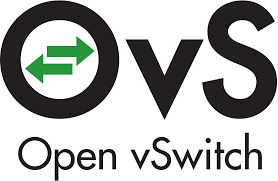
\includegraphics[scale=0.45]{ovs}
 \caption{OpenvSwitch logo}
 \label{chap:prjan:img:ovs_logo}
\end{figure}

\subsection{Floodlight}
\begin{figure}[h]
 \centering 
\includegraphics[scale=0.6]{floodlight}
 \caption{Floodlight logo}
 \label{chap:prjan:img:floodlight_logo}
\end{figure}

\subsection{Openbaton}
\begin{figure}[h]
  \centering \includegraphics[scale=0.45]{openbaton_logo}
  \caption{Openbaton logo}
  \label{chap:prjan:img:openbaton_logo}
\end{figure}